\documentclass[10pt,a4paper]{article}
\usepackage{graphicx}
\usepackage{subfig}
\usepackage{float}
\usepackage[english]{babel}
\usepackage[font=small,labelfont=bf]{caption}
\textwidth=450pt\oddsidemargin=0pt
\pagenumbering{arabic}

\begin{document}
\begin{titlepage}
\vspace{15mm}
\begin{center}
{\LARGE{\bf Andrea Leganza}}\\
\vspace{3mm}
{\LARGE{\bf MAT. 788513}}\\
\vspace{3mm}
{\LARGE{\bf\ }}\\
\end{center}
\vspace{40mm}
\par
\noindent
\begin{minipage}[t]{0.47\textwidth}
{\large{\bf}}
\end{minipage}
\hfill
\begin{center}
{\large{\bf Final homework }}
\end{center}
\vspace{20mm}
\begin{center}
{\large{\bf 09/09/2022}}
\end{center}
\end{titlepage}
\pagebreak


\section{Scene description}
The scene is a diorama of an island placed in the middle of the ocean, the scene can be switched to day and night mode showing/hiding different elements.

\section{Assets}

Props were mainly dowloaded from sketchfab.org website in GLTF format:

\begin{itemize}
 \item Castle
 \item Phoenix
 \item Boat
\end{itemize}

Most of the models required to be cleaned up, their structure and original materials to be modified too.

Leaves on the water were created using a simple transparent plane and applying on realtime downloaded textures, while fireflies where created using a plane with random color.

\section{User interface}

The GUI was developed using DAT.GUI, the whole interaction is controlled by javascript events. It provides controls to control all the aspect of the scene:
 
 \begin{itemize}
 \item Camera: position and rotation
 \item Controls: speed parameters, autorotate parameters
 \item Day/night switch, fog parameters, shadowmap on/off
 \item Ambient light: on/off, intensity and color
 \item Torches: on/off, animation, color, intensity
 \item Spotlight: on/off, shadows, color, intensity, distance, angle, penumbra, position
 \item Sky: on/off
 \item Water: on/off
 \item Particles: night fireflies on/off
 \item Postprocessing: on/off bloom/dof parameters
 \item Audio: on/off, volume
 \item Debug: on/off
 \end{itemize}
 
\begin{figure}[H]
\hfill
\subfloat[Menu]{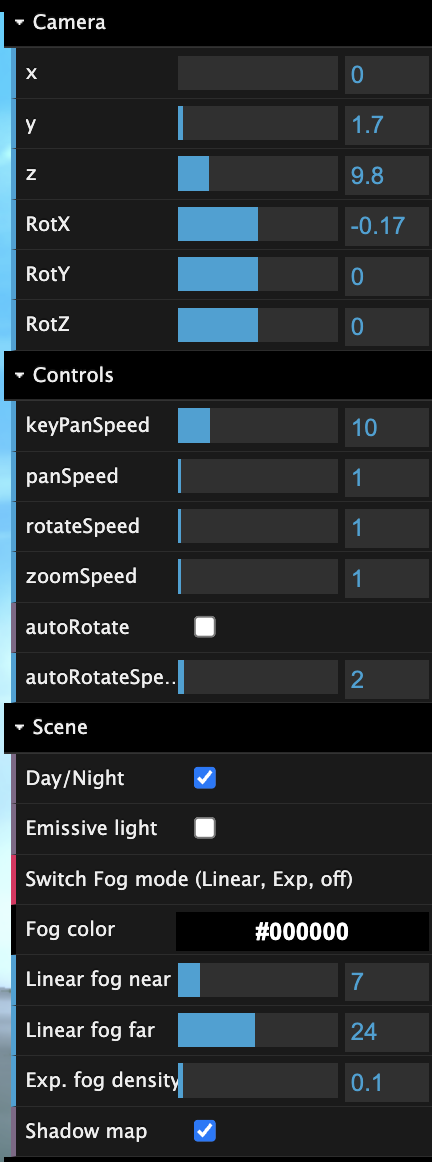
\includegraphics[width=3cm]{ui0}}
\hfill
\subfloat[Menu]{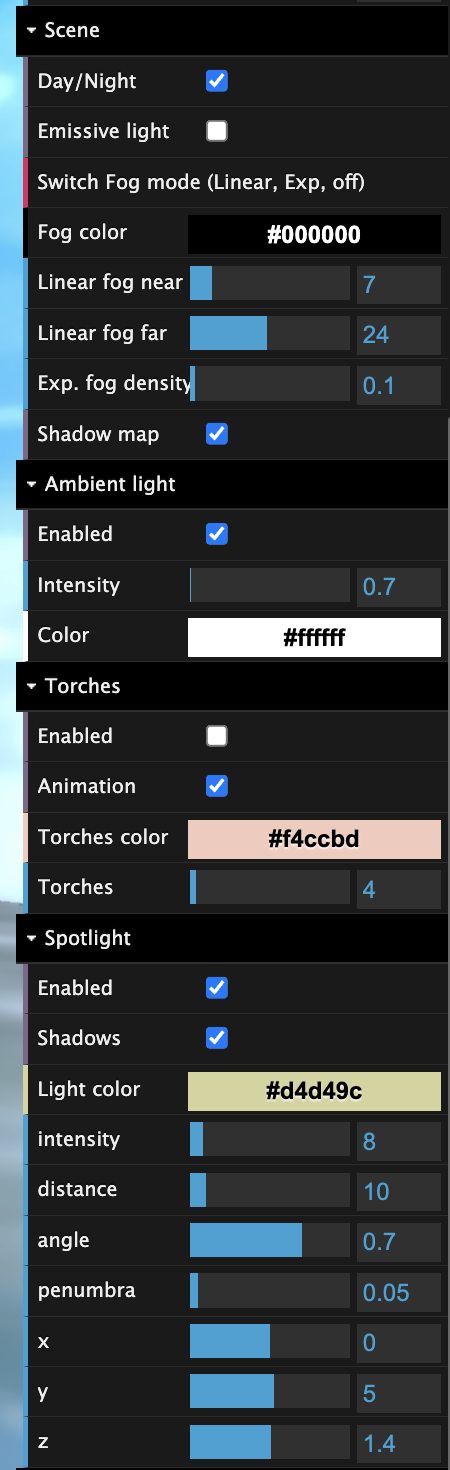
\includegraphics[width=3cm]{ui1}}
\hfill
\subfloat[Menu]{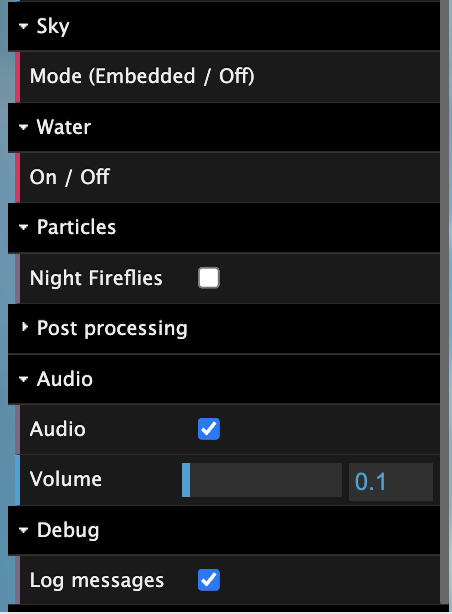
\includegraphics[width=3cm]{ui2}}
\hfill
\caption{Menu views}
\end{figure}

\section{Day/Night mode}

Switching to day/night mode using the GUI button lets to switch to different look of the scene, showing/hiding different elements:

\begin{itemize}
 \item Day: Phoenix flies around  the castle, sky rotates around, leaves float
 \item Night: A boat travels around the castle, night sky rotates, fireflies fly around, torches lights up and animate their flame, a crab eat and moves
\end{itemize}

\begin{itemize}
 \item The sky changes its texture from a cloudy day to a night sky.
 \item Fog changes to exp mode during night to increase the night look darkening the whole scene.
 \item Switching to night/day also customizes the lights with different colors and intensities to improve the scene look.
\end{itemize}
\begin{center}
\begin{figure}[H]
\caption{The DAY mode look}
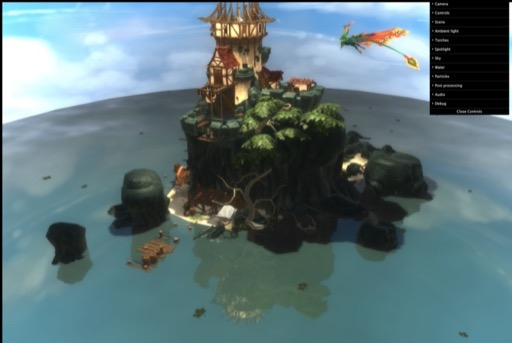
\includegraphics[width=1\textwidth,keepaspectratio]{day}
\caption{The NIGTH mode look}
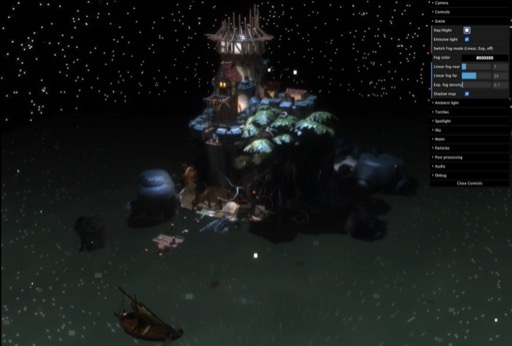
\includegraphics[width=1\textwidth,keepaspectratio]{night}
\end{figure}
\end{center}

\section{Torches}

\begin{figure}[H]
\caption{One of the torches}
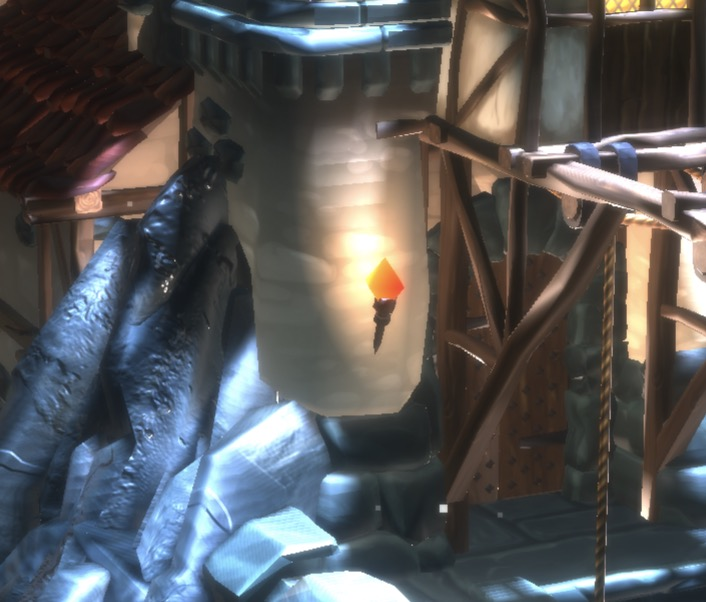
\includegraphics[width=0.8\textwidth]{torch}
\end{figure}


Torches are detected during mesh loading and to them are added:

\begin{itemize}
 \item A spotlight is added with related animation tween
 \item A sphere with some faces to mimic a Platonic solid to simulate the flame
\end{itemize}

To set the color of the flame a custom shader was made, which interpolates between two colors during the time (an uniform updated during the animation loop using a deltatime value) :

\begin{verbatim}
  const sphere = new THREE.SphereGeometry( 3, 4, 2 );

            const mat = new THREE.ShaderMaterial({
                uniforms: {
                    u_time: { type: "f", value: 0 }
                },
                vertexShader: `
                    varying vec2 vUv;
                    uniform float u_time;

                    void main() {
                        vUv = uv;

                        mat4 scale = mat4(vec4(1.0+sin(u_time)*0.1,0.0,0.0,0.0),
                                        vec4(0.0,1.0+sin(u_time)*0.3,0.0,0.0),
                                        vec4(0.0,0.0,1.0+sin(u_time)*0.5,0.0),
                                        vec4(0.0,0.0,0.0,1.0));
                        gl_Position = projectionMatrix * modelViewMatrix * scale * vec4(position,1.0);
                    }
                `,
                fragmentShader: `
                    uniform float u_time;
                    varying vec2 vUv;
                    
                    void main() {
                        gl_FragColor = vec4(mix(vec3(1,0,0), vec3(1,0.65,0), vUv.y+sin(u_time)), 1.0);
                    }
            `
            });
\end{verbatim}

\section{Leaves}

Leaves were created with a simple double side transparent plane, loading a random local stored leaf texture; their float around the scene with a simple Math.sin movement which starts from a random generated value written/readen using mesh userData in the animation loop.

\begin{center}
\begin{figure}[H]
  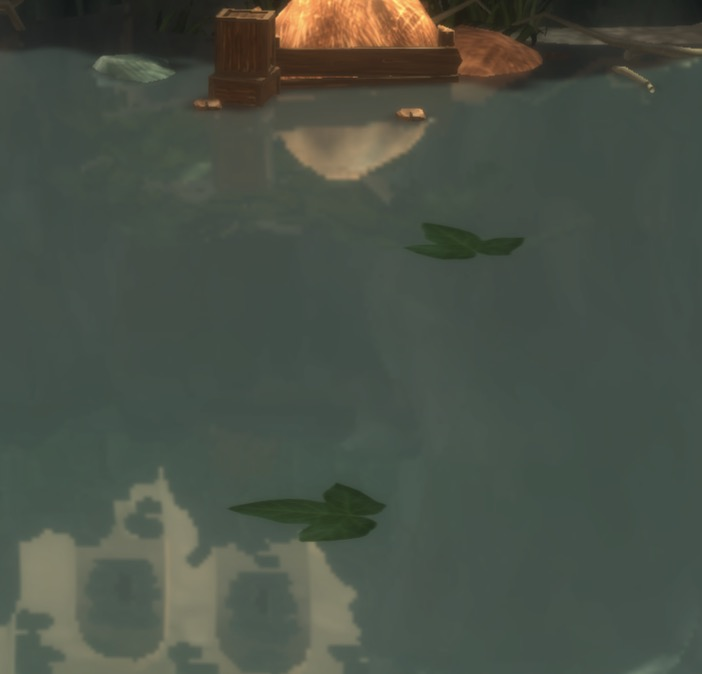
\includegraphics[width=0.5\textwidth]{leaves}
     \caption{The leaves on the surface}
\end{figure}
\end{center}

\begin{verbatim}
  const geometry = new THREE.PlaneGeometry( 1, 1 );
        const material = new THREE.MeshBasicMaterial( 
        {color: 0x263529, side: THREE.DoubleSide, depthTest: true, transparent: true} );

        const textureName = 'Textures/leaf'+(Math.floor(Math.random() * 3) + 0)+'.png';

        material.map = new THREE.TextureLoader().load( textureName , function  (texture) {
            texture.wrapS = texture.wrapT = THREE.RepeatWrapping;
        });
        
        var leavesCoordPosition = [];

        for (var i= 0; i <50;i++){
            var ranXNum = Math.ceil(Math.random() * 7) * (Math.round(Math.random()) ? 1 : -1)
            var ranYNum = Math.ceil(Math.random() * 7) * (Math.round(Math.random()) ? 1 : -1)

            const pos = new THREE.Vector3(ranXNum,ranYNum,0.1)
            leavesCoordPosition.push(pos);     
        }
    
        leavesCoordPosition.forEach(position => {

            if (debugMode){
                console.log(position);
            }
       
            const mesh = new THREE.Mesh( geometry, material );
            mesh.rotation.z = Math.random() * Math.PI * 2; 
            mesh.position.set(position.x,position.y,position.z);
          
            let s = Math.random() * 0.1 + 0.1;
            mesh.scale.set(s, s, s);
            mesh.userData.delta = Math.random() * Math.PI * 2;

            floatingObjects.push(mesh);
        
            if (water!=null){
                water.add(mesh);
            }
            else {
                sea.add(mesh)
            }

        });
\end{verbatim}

\section{Fireflies}

Fireflies were developed as simple squares of different sizes an colors embbeded inside a BufferGeometry with a PointsMaterial .

\begin{center}
\begin{figure}[H]
  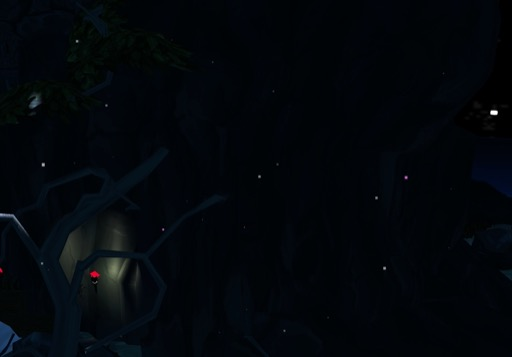
\includegraphics[width=0.5\textwidth]{fireflies}
     \caption{Fireflies flying around the night scene}
\end{figure}
\end{center}


\section{Animations}

Animations were implemented with different techniques:

\begin{itemize}
 \item Updating rotation/position properties of mesh directly
 \item Updating UV offset
 \item Using Tween.JS
 \item Updating shader properties
\end{itemize}

\bigbreak

The following elements were animated:
\begin{itemize}
 \item Sky: rotates on z axis on day, on z and y axis during night
 \item Water: translates up/down to simulate low/high tide
 \item Torches: flame scales and rotates, their lights glow randomly
 \item Leaves on the water: oscillate on the surface
 \item Phoenix (day mode) flies and rotate around a spline (CatmullRomCurve3)
 \item Boat (night mode) rotate around castle and floats up/down
 \item Boat lantern: oscillates
 \item Crab: every leg moves, claws move, crab moves left/right, crab lookA the camera
 \item Fireflies particles: randomly move
 \end{itemize}

\section{Phoenix}

The original model was rigged and was a sigle mesh, the first operation that was done on it was to remove the whole rigging hierarchy and split the different segments in Blender, then a proper hierarchy was created starting  from the body. To speed up the animation process "custom properties" were  added to each of the mesh segments to pass axis, easing, delay and movement direction which were read in three.js by accessing the userdata property; these properties were then used by Tween.js to animate as needed. All the meshes required to set an ad hoc pivot to be properly aimated.

\begin{figure}[H]
   \caption{The phoenix structure}
  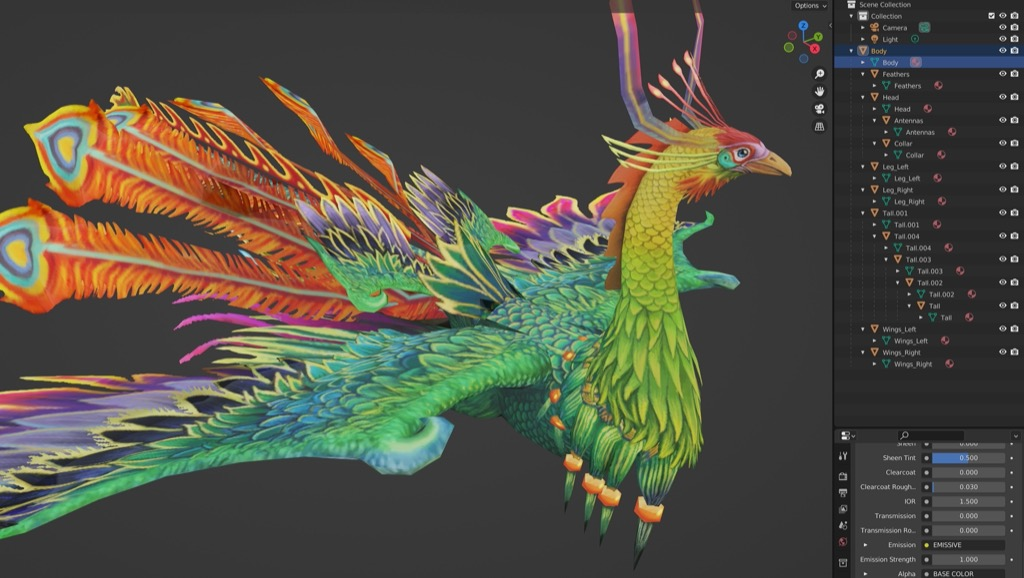
\includegraphics[width=1\textwidth]{phoenix}
\end{figure}

\begin{figure}[H]
\caption{Custom properties used to pass data to Three.js}
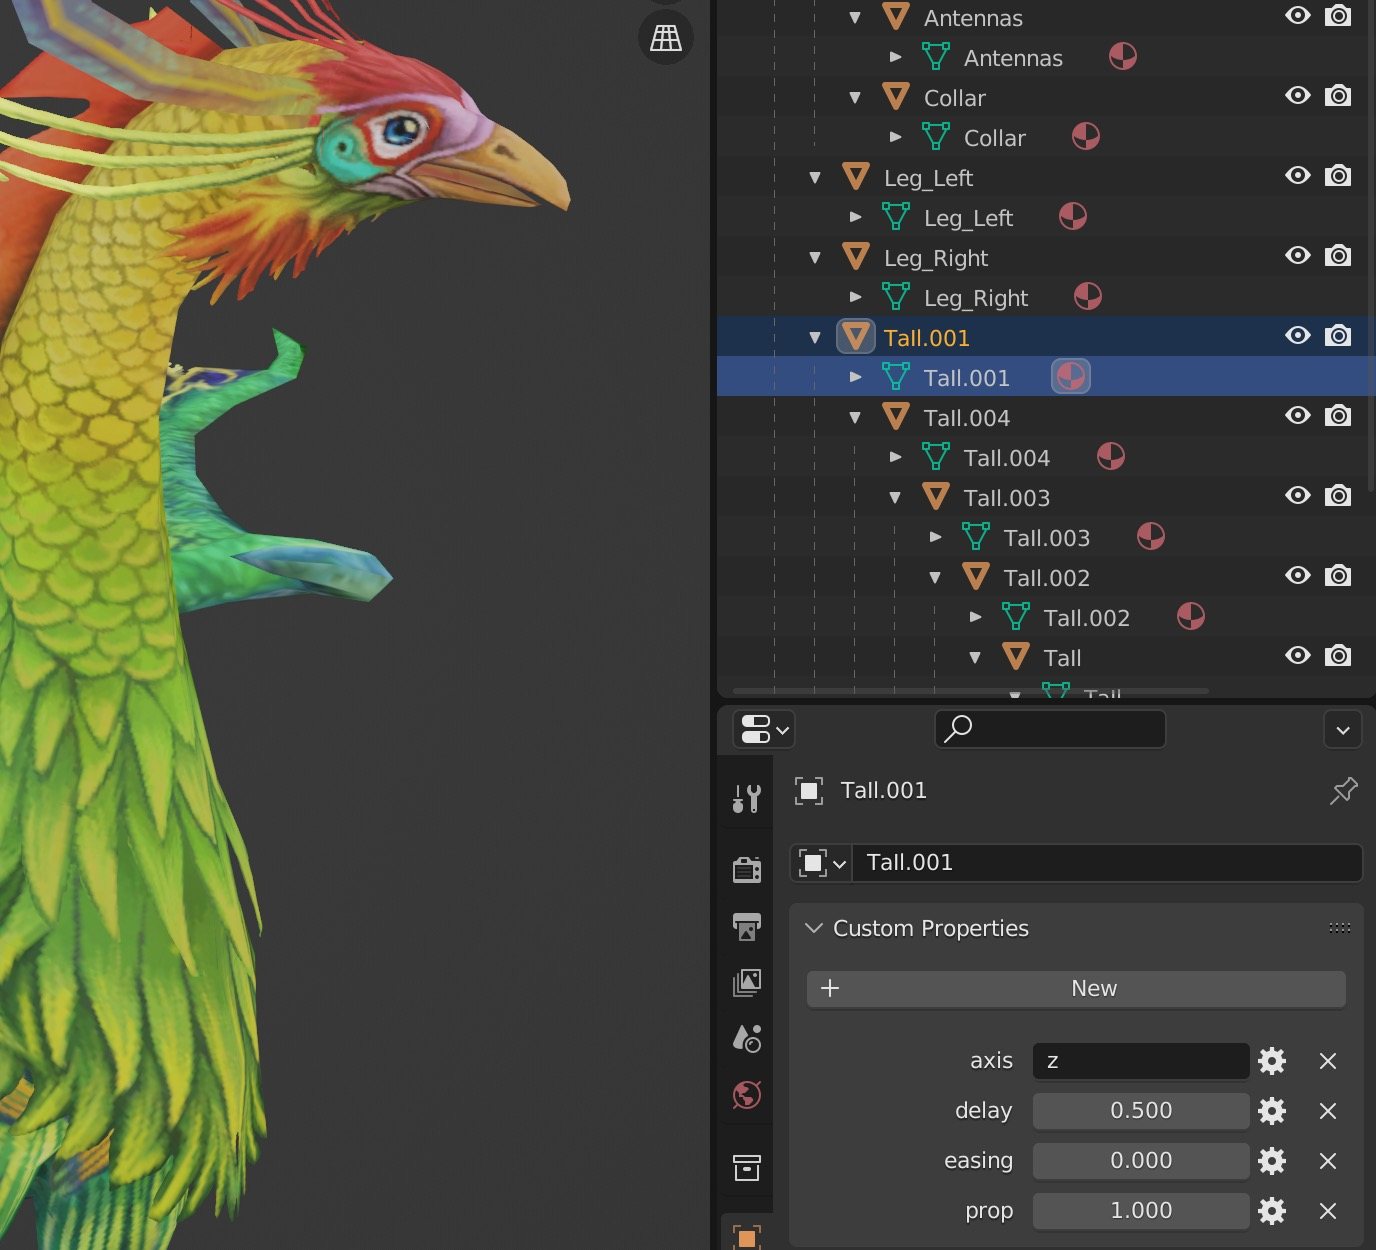
\includegraphics[width=1\textwidth]{phoenix_data}
\end{figure}

\section{Boat}

The boat was cleaned up, the pivot was changed to a proper position, the lantern was separated from the boat and the pivot set in the correct position for both of them to proper support the animation process.

\begin{center}
\begin{figure}[H]
\caption{The boat structure}
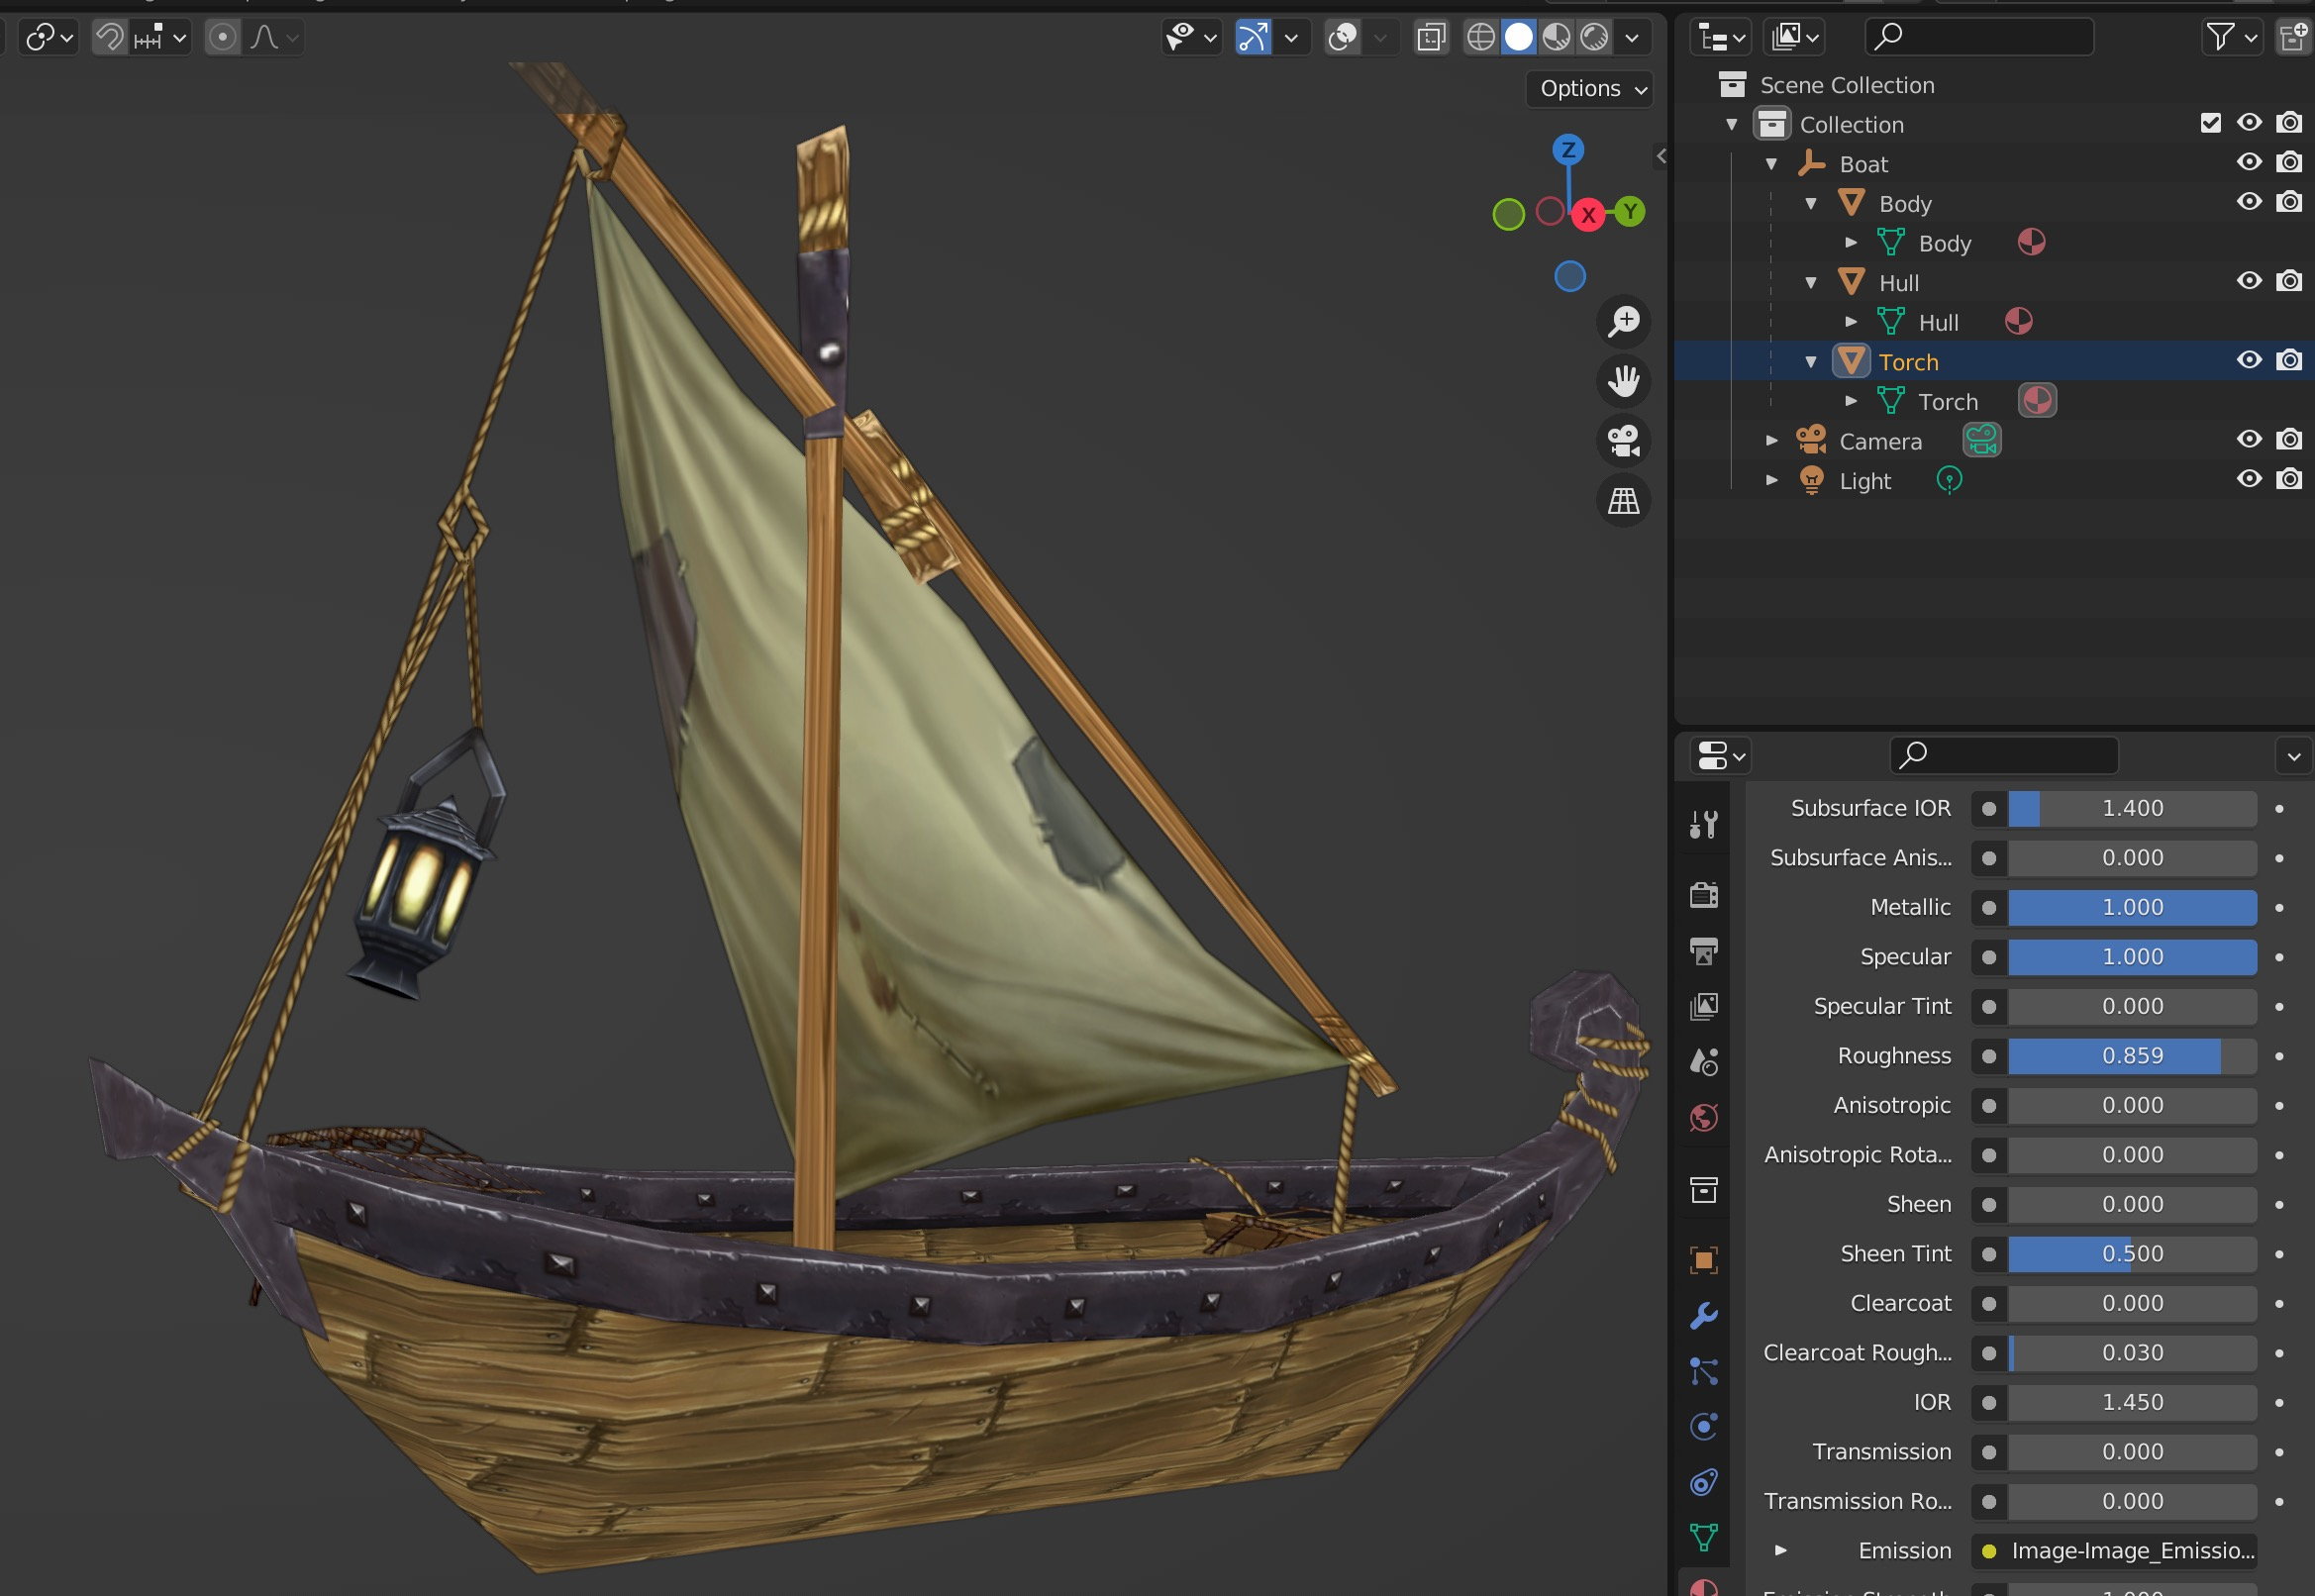
\includegraphics[width=1\textwidth]{boat}
\end{figure}
\end{center}


\section{Crab}

The crab was cleaned up, the mesh was reduced using Blender modifier, the pivot was changed to a proper position for each segment, crab legs are animated using Tween.js usig the same approach of the Phoenix usig model custom properties.

\begin{center}
\begin{figure}[H]
\caption{The crab structure}
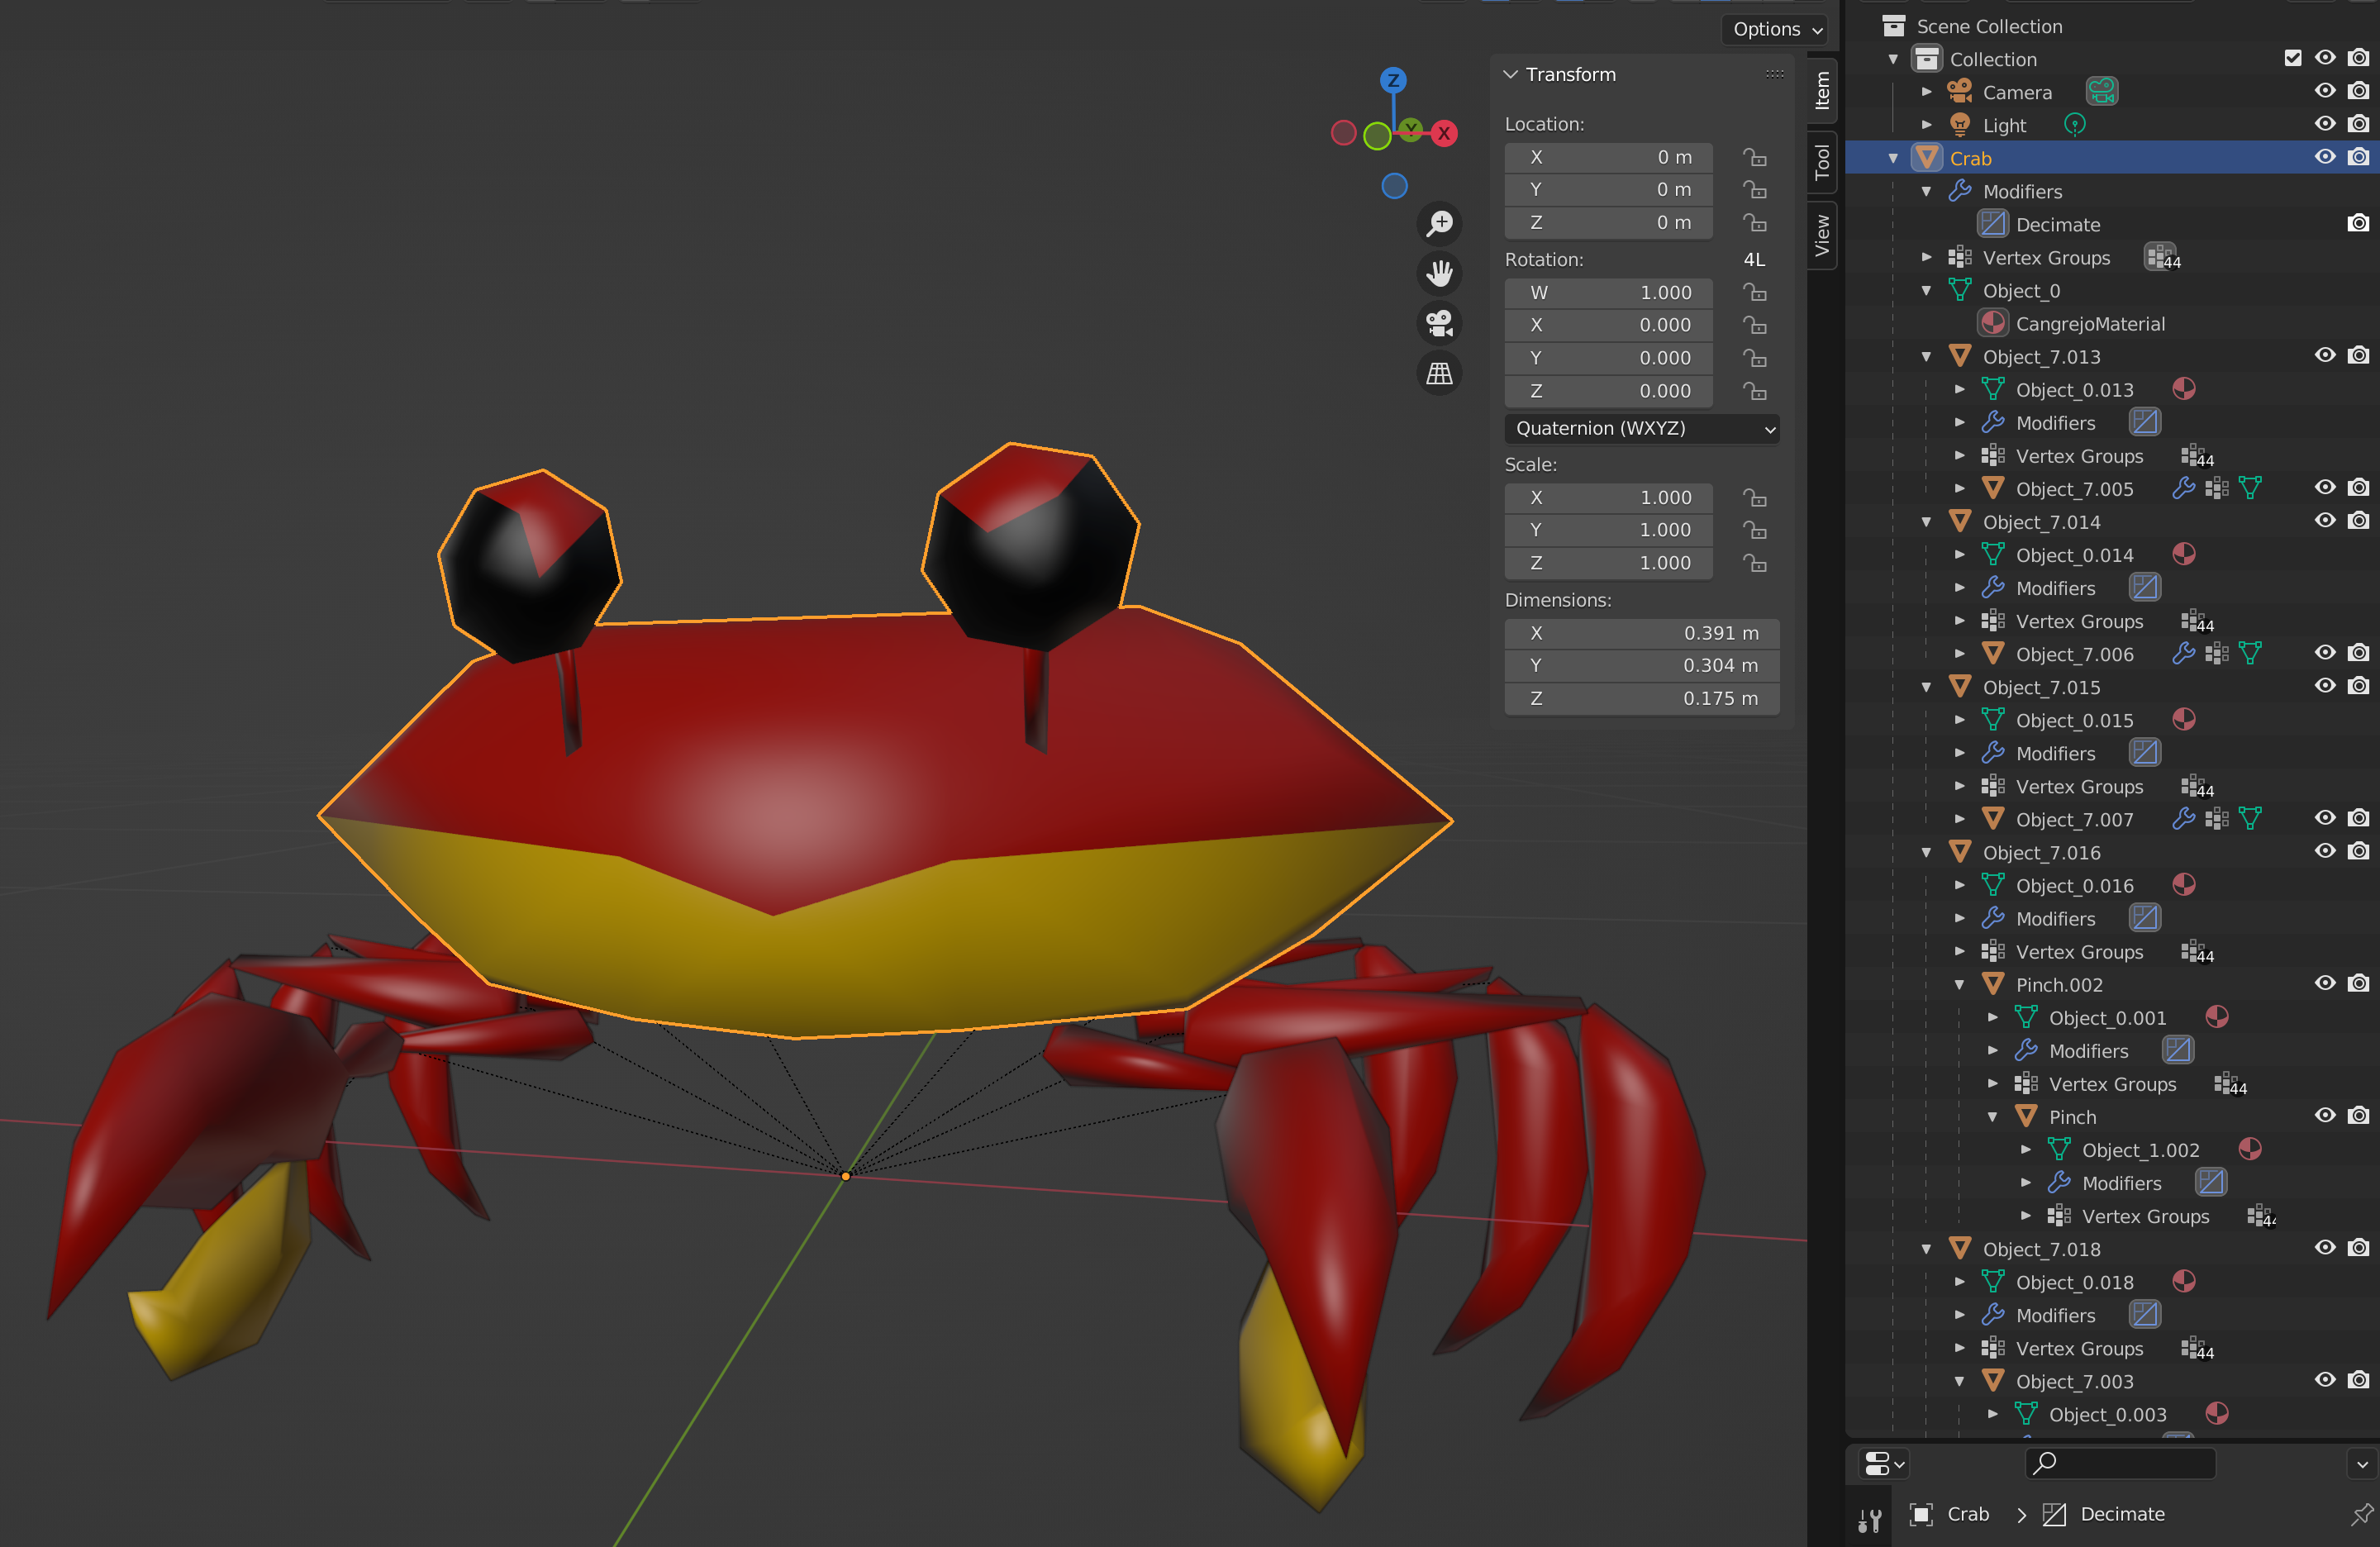
\includegraphics[width=1\textwidth]{crab}
\end{figure}
\end{center}


\section{Textures}
The following textures were used:

\begin{itemize}
\item Base/Albedo map
\item Normal map
\item Emissive map
\end{itemize}

For some models the normal map was generated from base/albedo map using an online tool; for emission some maps were generated by hand modifying in Krita the base map; the emissive intensity effect was increased during the load of the models and a GUI option is available to change its value.

\section{Lights}
The lights used in the scene are different:

\begin{itemize}
\item An Ambient Light to light the whole scene
\item A Spotlight to light from the top the castle
\item Point lights for each torch lights to simulate the light of the torches
\end{itemize}

\section{Audio}

A seashore audio loop sound effect is provided, during the day mode a seagull sound is played too, while during the night a crickets soud is played.

\section{Notes}

The performances during camera look aren't great, performances should be improved  using lightmapping, storing shadows and reducing polygon count.

\end{document}

